\documentclass{article}
\usepackage{tikz, comment}
\usepackage{pifont}
\usepackage{fontspec, pgfplots}
\usetikzlibrary{arrows, decorations.markings, decorations.pathreplacing}
\begin{comment}
:Title: Not defined yet
:Tags: absolute value rules;properties of equality, equation rules;equivalence properties of equality;proper subset;trichotomy
:Prob: 0.7297;0.6321;0.5683;0.5626;0.559
:Author: Prof.Hu Ji-shan, HKUST
:Slug: No name yet

Description Here.........
\end{comment}
\begin{document}\centering 

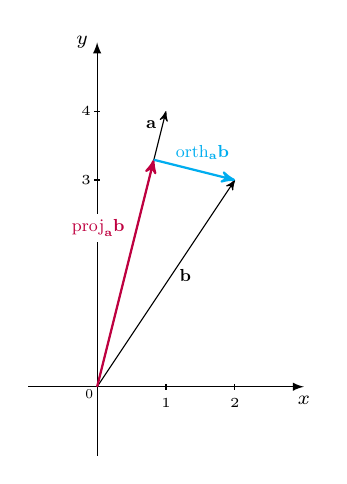
\begin{tikzpicture}[>=latex,xscale=.5*1.75, yscale=.5*1.75][font=\sf\small] 

%\draw[xstep=1cm,ystep=1cm,color=gray!80] (0, -1) grid (8, 8);

    	\foreach \x in {1, 2}
     		\draw (\x,2pt/1.75) -- (\x,-2pt/1.75)
			node[anchor=north] {\tiny$\x$}
			;

    	\foreach \x in {}
     		\draw (\x,2pt/1) -- (\x,-2pt/1)
			node[anchor=south] {\tiny$\x$}
			;
    	\foreach \y in {3, 4}
     		\draw (-2pt/1.75,\y) -- (2pt/1.75,\y)
			node[anchor=east] {\tiny $\y$}
			;

\draw[->] (-1, 0) -- (3, 0)node[below] {\scriptsize$x$} ;
\draw[->] (0, -1) -- (0, 5)node[left] {\scriptsize$y$} ;

\draw[->, >=stealth'] (0, 0) -- (2, 3)node[black, below, midway, pos=0.6, xshift=2, yshift=0, scale=0.7]{${\bf b}$};

\draw[->, >=stealth'] (0, 0) -- (1, 4)node[black, left, midway, pos=0.95, xshift=0, yshift=0, scale=0.7]{${\bf a}$};

\draw[purple, thick, ->, >=stealth'] (0, 0) -- ({14/17}, {56/17})node[left, fill=white, midway, pos=0.7, xshift=-2, yshift=0, scale=0.7]{$\hbox{\rm proj}_{\bf a} {\bf b}$};

\draw[cyan, thick, ->, >=stealth'] ({14/17}, {56/17})--({20/17+14/17},{-5/17+56/17})node[above, midway, pos=0.6, xshift=0, yshift=2, scale=0.7]{$\hbox{\rm orth}_{\bf a} {\bf b}$};

\node[scale=0.7] at (-0.2/1.75, -0.2/1.75) {\scriptsize$0$};

\end{tikzpicture}
\end{document}